\documentclass{standalone}
\usepackage[utf8]{inputenc}
\usepackage{lmodern}
\usepackage[T1]{fontenc}

\usepackage{amssymb,amsmath,amsthm,amsfonts}
\usepackage{mathtools}
\usepackage{commath}
\usepackage{dsfont}
\usepackage{calrsfs}
\DeclareMathAlphabet{\pazocal}{OMS}{zplm}{m}{n}
\usepackage{stmaryrd}
\usepackage{etoolbox}

\usepackage{booktabs}

\usepackage{xcolor}
\usepackage{pgfplots}
	\pgfplotsset{compat=1.16}
	\usetikzlibrary{decorations.pathreplacing}

\usepackage[textsize=footnotesize]{todonotes}
\setlength{\marginparwidth}{2cm}

\begin{document}
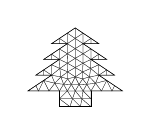
\begin{tikzpicture}[scale=1, line width=0.1pt]
\draw[fill=none, draw=black!75](-0.20000,0.00000) --(-0.06667,0.00000) --(-0.20000,0.10000) -- cycle;
\draw[fill=none, draw=black!75](-0.06667,0.00000) --(0.06667,0.00000) --(-0.03447,0.10055) -- cycle;
\draw[fill=none, draw=black!75](0.20000,0.00000) --(0.08461,0.10009) --(0.06667,0.00000) -- cycle;
\draw[fill=none, draw=black!75](0.06667,0.00000) --(0.08461,0.10009) --(-0.03447,0.10055) -- cycle;
\draw[fill=none, draw=black!75](0.20000,0.00000) --(0.20000,0.10000) --(0.08461,0.10009) -- cycle;
\draw[fill=none, draw=black!75](0.20000,0.20000) --(0.10000,0.20000) --(0.20000,0.10000) -- cycle;
\draw[fill=none, draw=black!75](0.20000,0.10000) --(0.10000,0.20000) --(0.08461,0.10009) -- cycle;
\draw[fill=none, draw=black!75](0.00000,0.20000) --(0.08461,0.10009) --(0.10000,0.20000) -- cycle;
\draw[fill=none, draw=black!75](0.00000,0.20000) --(-0.10000,0.20000) --(-0.03447,0.10055) -- cycle;
\draw[fill=none, draw=black!75](-0.20000,0.20000) --(-0.20000,0.10000) --(-0.10000,0.20000) -- cycle;
\draw[fill=none, draw=black!75](0.00000,0.20000) --(-0.03447,0.10055) --(0.08461,0.10009) -- cycle;
\draw[fill=none, draw=black!75](-0.06667,0.00000) --(-0.03447,0.10055) --(-0.20000,0.10000) -- cycle;
\draw[fill=none, draw=black!75](-0.10000,0.20000) --(-0.20000,0.10000) --(-0.03447,0.10055) -- cycle;
\draw[fill=none, draw=black!75](0.20000,0.20000) --(0.14718,0.28459) --(0.10000,0.20000) -- cycle;
\draw[fill=none, draw=black!75](0.00000,0.20000) --(0.10000,0.20000) --(0.04865,0.28197) -- cycle;
\draw[fill=none, draw=black!75](0.10000,0.20000) --(0.14718,0.28459) --(0.04865,0.28197) -- cycle;
\draw[fill=none, draw=black!75](0.00000,0.20000) --(-0.04865,0.28197) --(-0.10000,0.20000) -- cycle;
\draw[fill=none, draw=black!75](0.00000,0.20000) --(0.04865,0.28197) --(-0.04865,0.28197) -- cycle;
\draw[fill=none, draw=black!75](-0.20000,0.20000) --(-0.10000,0.20000) --(-0.14719,0.28459) -- cycle;
\draw[fill=none, draw=black!75](-0.10000,0.20000) --(-0.04865,0.28197) --(-0.14719,0.28459) -- cycle;
\draw[fill=none, draw=black!75](0.60000,0.20000) --(0.50000,0.26667) --(0.46667,0.20000) -- cycle;
\draw[fill=none, draw=black!75](-0.00001,0.37861) --(0.09536,0.44228) --(-0.00001,0.49689) -- cycle;
\draw[fill=none, draw=black!75](0.46667,0.20000) --(0.50000,0.26667) --(0.40000,0.33333) -- cycle;
\draw[fill=none, draw=black!75](0.30000,0.40000) --(0.25884,0.29742) --(0.40000,0.33333) -- cycle;
\draw[fill=none, draw=black!75](0.09851,0.55177) --(-0.00001,0.49689) --(0.09536,0.44228) -- cycle;
\draw[fill=none, draw=black!75](0.50000,0.40000) --(0.40000,0.46667) --(0.40000,0.40000) -- cycle;
\draw[fill=none, draw=black!75](0.20000,0.60000) --(0.19557,0.48530) --(0.30000,0.53333) -- cycle;
\draw[fill=none, draw=black!75](0.40000,0.60000) --(0.30000,0.66667) --(0.30000,0.60000) -- cycle;
\draw[fill=none, draw=black!75](0.10000,0.80000) --(0.09980,0.67264) --(0.20000,0.73333) -- cycle;
\draw[fill=none, draw=black!75](0.30000,0.80000) --(0.20000,0.86667) --(0.20000,0.80000) -- cycle;
\draw[fill=none, draw=black!75](0.00000,1.00000) --(-0.00000,0.86718) --(0.10000,0.93333) -- cycle;
\draw[fill=none, draw=black!75](0.00000,1.00000) --(-0.10000,0.93333) --(-0.00000,0.86718) -- cycle;
\draw[fill=none, draw=black!75](-0.60000,0.20000) --(-0.46667,0.20000) --(-0.50000,0.26667) -- cycle;
\draw[fill=none, draw=black!75](-0.00001,0.37861) --(-0.00001,0.49689) --(-0.09537,0.44228) -- cycle;
\draw[fill=none, draw=black!75](-0.46667,0.20000) --(-0.40000,0.33333) --(-0.50000,0.26667) -- cycle;
\draw[fill=none, draw=black!75](-0.30000,0.40000) --(-0.40000,0.33333) --(-0.25885,0.29742) -- cycle;
\draw[fill=none, draw=black!75](-0.00001,0.37861) --(0.09476,0.35340) --(0.09536,0.44228) -- cycle;
\draw[fill=none, draw=black!75](-0.50000,0.40000) --(-0.40000,0.40000) --(-0.40000,0.46667) -- cycle;
\draw[fill=none, draw=black!75](-0.20000,0.60000) --(-0.30000,0.53333) --(-0.19558,0.48530) -- cycle;
\draw[fill=none, draw=black!75](-0.40000,0.60000) --(-0.30000,0.60000) --(-0.30000,0.66667) -- cycle;
\draw[fill=none, draw=black!75](-0.10000,0.80000) --(-0.20000,0.73333) --(-0.09980,0.67264) -- cycle;
\draw[fill=none, draw=black!75](-0.30000,0.80000) --(-0.20000,0.80000) --(-0.20000,0.86667) -- cycle;
\draw[fill=none, draw=black!75](0.30000,0.40000) --(0.40000,0.40000) --(0.40000,0.46667) -- cycle;
\draw[fill=none, draw=black!75](0.20000,0.60000) --(0.30000,0.60000) --(0.30000,0.66667) -- cycle;
\draw[fill=none, draw=black!75](0.10000,0.80000) --(0.20000,0.80000) --(0.20000,0.86667) -- cycle;
\draw[fill=none, draw=black!75](-0.30000,0.40000) --(-0.40000,0.46667) --(-0.40000,0.40000) -- cycle;
\draw[fill=none, draw=black!75](-0.20000,0.60000) --(-0.30000,0.66667) --(-0.30000,0.60000) -- cycle;
\draw[fill=none, draw=black!75](-0.10000,0.80000) --(-0.20000,0.86667) --(-0.20000,0.80000) -- cycle;
\draw[fill=none, draw=black!75](0.30000,0.40000) --(0.40000,0.46667) --(0.30000,0.53333) -- cycle;
\draw[fill=none, draw=black!75](0.20000,0.60000) --(0.30000,0.66667) --(0.20000,0.73333) -- cycle;
\draw[fill=none, draw=black!75](0.20000,0.60000) --(0.20000,0.73333) --(0.09980,0.67264) -- cycle;
\draw[fill=none, draw=black!75](0.10000,0.80000) --(0.20000,0.86667) --(0.10000,0.93333) -- cycle;
\draw[fill=none, draw=black!75](0.10000,0.80000) --(0.10000,0.93333) --(-0.00000,0.86718) -- cycle;
\draw[fill=none, draw=black!75](-0.30000,0.40000) --(-0.30000,0.53333) --(-0.40000,0.46667) -- cycle;
\draw[fill=none, draw=black!75](-0.30000,0.40000) --(-0.19558,0.48530) --(-0.30000,0.53333) -- cycle;
\draw[fill=none, draw=black!75](-0.20000,0.60000) --(-0.20000,0.73333) --(-0.30000,0.66667) -- cycle;
\draw[fill=none, draw=black!75](-0.20000,0.60000) --(-0.09980,0.67264) --(-0.20000,0.73333) -- cycle;
\draw[fill=none, draw=black!75](-0.10000,0.80000) --(-0.10000,0.93333) --(-0.20000,0.86667) -- cycle;
\draw[fill=none, draw=black!75](-0.10000,0.80000) --(-0.00000,0.86718) --(-0.10000,0.93333) -- cycle;
\draw[fill=none, draw=black!75](0.30000,0.40000) --(0.30000,0.53333) --(0.19557,0.48530) -- cycle;
\draw[fill=none, draw=black!75](-0.20000,0.20000) --(-0.14719,0.28459) --(-0.25885,0.29742) -- cycle;
\draw[fill=none, draw=black!75](0.20000,0.20000) --(0.33333,0.20000) --(0.25884,0.29742) -- cycle;
\draw[fill=none, draw=black!75](0.33333,0.20000) --(0.46667,0.20000) --(0.40000,0.33333) -- cycle;
\draw[fill=none, draw=black!75](0.30000,0.40000) --(0.18184,0.37795) --(0.25884,0.29742) -- cycle;
\draw[fill=none, draw=black!75](0.30000,0.40000) --(0.19557,0.48530) --(0.18184,0.37795) -- cycle;
\draw[fill=none, draw=black!75](0.20000,0.60000) --(0.09851,0.55177) --(0.19557,0.48530) -- cycle;
\draw[fill=none, draw=black!75](0.20000,0.60000) --(0.09980,0.67264) --(0.09851,0.55177) -- cycle;
\draw[fill=none, draw=black!75](0.10000,0.80000) --(-0.00000,0.86718) --(-0.00000,0.73745) -- cycle;
\draw[fill=none, draw=black!75](0.10000,0.80000) --(-0.00000,0.73745) --(0.09980,0.67264) -- cycle;
\draw[fill=none, draw=black!75](-0.10000,0.80000) --(-0.00000,0.73745) --(-0.00000,0.86718) -- cycle;
\draw[fill=none, draw=black!75](-0.20000,0.20000) --(-0.25885,0.29742) --(-0.33333,0.20000) -- cycle;
\draw[fill=none, draw=black!75](-0.33333,0.20000) --(-0.40000,0.33333) --(-0.46667,0.20000) -- cycle;
\draw[fill=none, draw=black!75](-0.20000,0.60000) --(-0.19558,0.48530) --(-0.09852,0.55177) -- cycle;
\draw[fill=none, draw=black!75](-0.20000,0.60000) --(-0.09852,0.55177) --(-0.09980,0.67264) -- cycle;
\draw[fill=none, draw=black!75](-0.30000,0.40000) --(-0.18185,0.37794) --(-0.19558,0.48530) -- cycle;
\draw[fill=none, draw=black!75](-0.30000,0.40000) --(-0.25885,0.29742) --(-0.18185,0.37794) -- cycle;
\draw[fill=none, draw=black!75](-0.10000,0.80000) --(-0.09980,0.67264) --(-0.00000,0.73745) -- cycle;
\draw[fill=none, draw=black!75](0.20000,0.20000) --(0.25884,0.29742) --(0.14718,0.28459) -- cycle;
\draw[fill=none, draw=black!75](0.04865,0.28197) --(-0.00001,0.37861) --(-0.04865,0.28197) -- cycle;
\draw[fill=none, draw=black!75](0.33333,0.20000) --(0.40000,0.33333) --(0.25884,0.29742) -- cycle;
\draw[fill=none, draw=black!75](0.14718,0.28459) --(0.25884,0.29742) --(0.18184,0.37795) -- cycle;
\draw[fill=none, draw=black!75](-0.33333,0.20000) --(-0.25885,0.29742) --(-0.40000,0.33333) -- cycle;
\draw[fill=none, draw=black!75](0.09980,0.67264) --(-0.00000,0.73745) --(-0.00000,0.61370) -- cycle;
\draw[fill=none, draw=black!75](0.09980,0.67264) --(-0.00000,0.61370) --(0.09851,0.55177) -- cycle;
\draw[fill=none, draw=black!75](-0.09980,0.67264) --(-0.00000,0.61370) --(-0.00000,0.73745) -- cycle;
\draw[fill=none, draw=black!75](-0.14719,0.28459) --(-0.18185,0.37794) --(-0.25885,0.29742) -- cycle;
\draw[fill=none, draw=black!75](0.14718,0.28459) --(0.09476,0.35340) --(0.04865,0.28197) -- cycle;
\draw[fill=none, draw=black!75](0.04865,0.28197) --(0.09476,0.35340) --(-0.00001,0.37861) -- cycle;
\draw[fill=none, draw=black!75](0.14718,0.28459) --(0.18184,0.37795) --(0.09476,0.35340) -- cycle;
\draw[fill=none, draw=black!75](-0.04865,0.28197) --(-0.09477,0.35340) --(-0.14719,0.28459) -- cycle;
\draw[fill=none, draw=black!75](-0.14719,0.28459) --(-0.09477,0.35340) --(-0.18185,0.37794) -- cycle;
\draw[fill=none, draw=black!75](-0.04865,0.28197) --(-0.00001,0.37861) --(-0.09477,0.35340) -- cycle;
\draw[fill=none, draw=black!75](0.19557,0.48530) --(0.09536,0.44228) --(0.18184,0.37795) -- cycle;
\draw[fill=none, draw=black!75](0.18184,0.37795) --(0.09536,0.44228) --(0.09476,0.35340) -- cycle;
\draw[fill=none, draw=black!75](0.19557,0.48530) --(0.09851,0.55177) --(0.09536,0.44228) -- cycle;
\draw[fill=none, draw=black!75](-0.09980,0.67264) --(-0.09852,0.55177) --(-0.00000,0.61370) -- cycle;
\draw[fill=none, draw=black!75](-0.19558,0.48530) --(-0.18185,0.37794) --(-0.09537,0.44228) -- cycle;
\draw[fill=none, draw=black!75](-0.19558,0.48530) --(-0.09537,0.44228) --(-0.09852,0.55177) -- cycle;
\draw[fill=none, draw=black!75](-0.18185,0.37794) --(-0.09477,0.35340) --(-0.09537,0.44228) -- cycle;
\draw[fill=none, draw=black!75](-0.09852,0.55177) --(-0.00001,0.49689) --(-0.00000,0.61370) -- cycle;
\draw[fill=none, draw=black!75](0.09851,0.55177) --(-0.00000,0.61370) --(-0.00001,0.49689) -- cycle;
\draw[fill=none, draw=black!75](-0.09852,0.55177) --(-0.09537,0.44228) --(-0.00001,0.49689) -- cycle;
\draw[fill=none, draw=black!75](-0.00001,0.37861) --(-0.09537,0.44228) --(-0.09477,0.35340) -- cycle;
\draw[black,line width=0.2pt] (-0.2,0.2) -- (-0.2,0) -- (0.2,0) -- (0.2,0.2);
\draw[black,line width=0.2pt] (0.2,0.2) -- (0.6,0.2) -- (0.3,0.4) -- (0.5,0.4) -- (0.2,0.6) -- (0.4,0.6) -- (0.1,0.8) -- (0.3,0.8) -- (0,1);
\draw[black,line width=0.2pt] (-0.2,0.2) -- (-0.6,0.2) -- (-0.3,0.4) -- (-0.5,0.4) -- (-0.2,0.6) -- (-0.4,0.6) -- (-0.1,0.8) -- (-0.3,0.8) -- (0,1);

\end{tikzpicture}

\end{document}

